\documentclass{minimal}
\usepackage{tikz}
\usetikzlibrary{calc,matrix}
 
\begin{document}
\let\vec\mathbf
   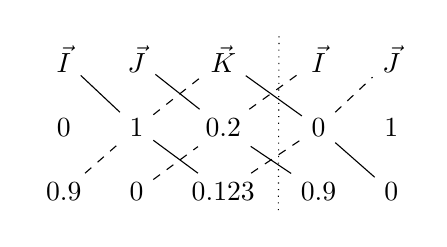
\begin{tikzpicture}
     \matrix [%
       matrix of math nodes,
       column sep=1em,
       row sep=1em
     ] (sarrus) {%
       \vec{I} & \vec{J} & \vec{K} & \vec{I} & \vec{J} \\
               0 &          1 &       0.2 &         0 &           1 \\
            0.9 &          0 &   0.123 &      0.9 &           0 \\
     }; 
 
     \path ($(sarrus-1-3.north east)+(1.2em,0)$) edge[dotted] ($(sarrus-3-3.south east)+(0.5em,0)$)
           (sarrus-1-1)                          edge         (sarrus-2-2)
           (sarrus-2-2)                          edge         (sarrus-3-3)
           (sarrus-1-2)                          edge         (sarrus-2-3)
           (sarrus-2-3)                          edge         (sarrus-3-4)
           (sarrus-1-3)                          edge         (sarrus-2-4)
           (sarrus-2-4)                          edge         (sarrus-3-5)
           (sarrus-3-1)                          edge[dashed] (sarrus-2-2)
           (sarrus-2-2)                          edge[dashed] (sarrus-1-3)
           (sarrus-3-2)                          edge[dashed] (sarrus-2-3)
           (sarrus-2-3)                          edge[dashed] (sarrus-1-4)
           (sarrus-3-3)                          edge[dashed] (sarrus-2-4)
           (sarrus-2-4)                          edge[dashed] (sarrus-1-5);
 
    
   \end{tikzpicture}
\end{document}